\section{Object 9}
\markright{Object 9}

To create this component, the Revolved Boss/Base feature was employed. The key step was designing a precise 2D sketch that defined the part's cross-section. Once fully defined, this sketch was revolved around a vertical axis to produce the final three-dimensional shape, demonstrating an efficient method for creating parts with rotational symmetry.

\begin{figure}[H]
	\centering

	\begin{subfigure}[b]{0.49\textwidth}
		\centering
		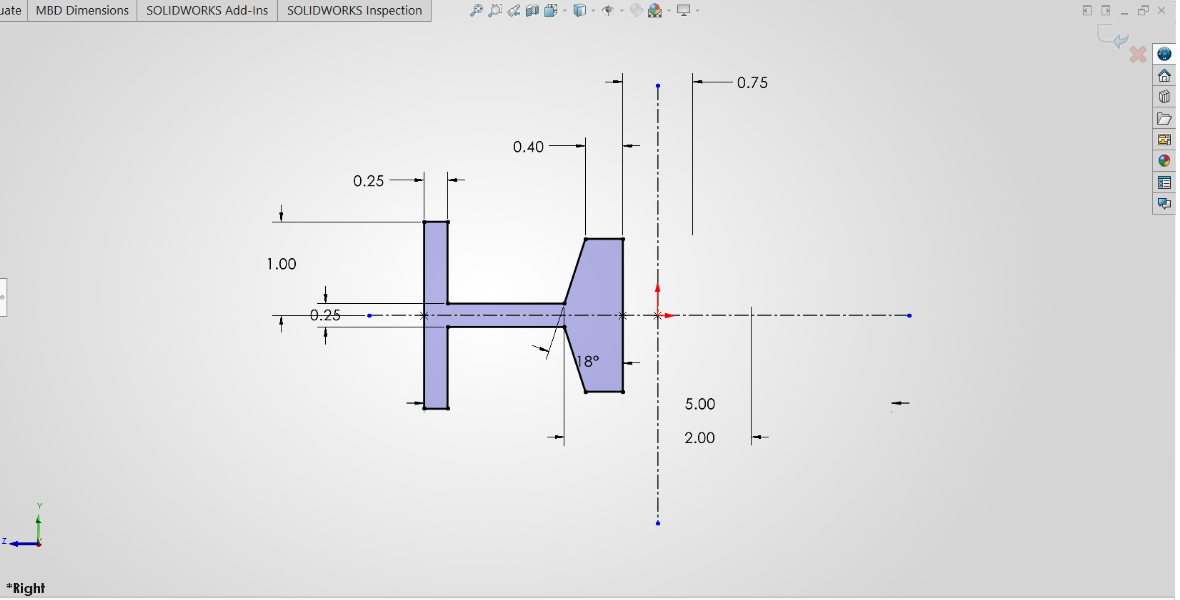
\includegraphics[width=\textwidth, keepaspectratio]{lab-01/assets/object-9/object-9-snap-1.png}
		\caption{2D sketch with dimensions.}
	\end{subfigure}%
	\hfill
	\begin{subfigure}[b]{0.49\textwidth}
		\centering
		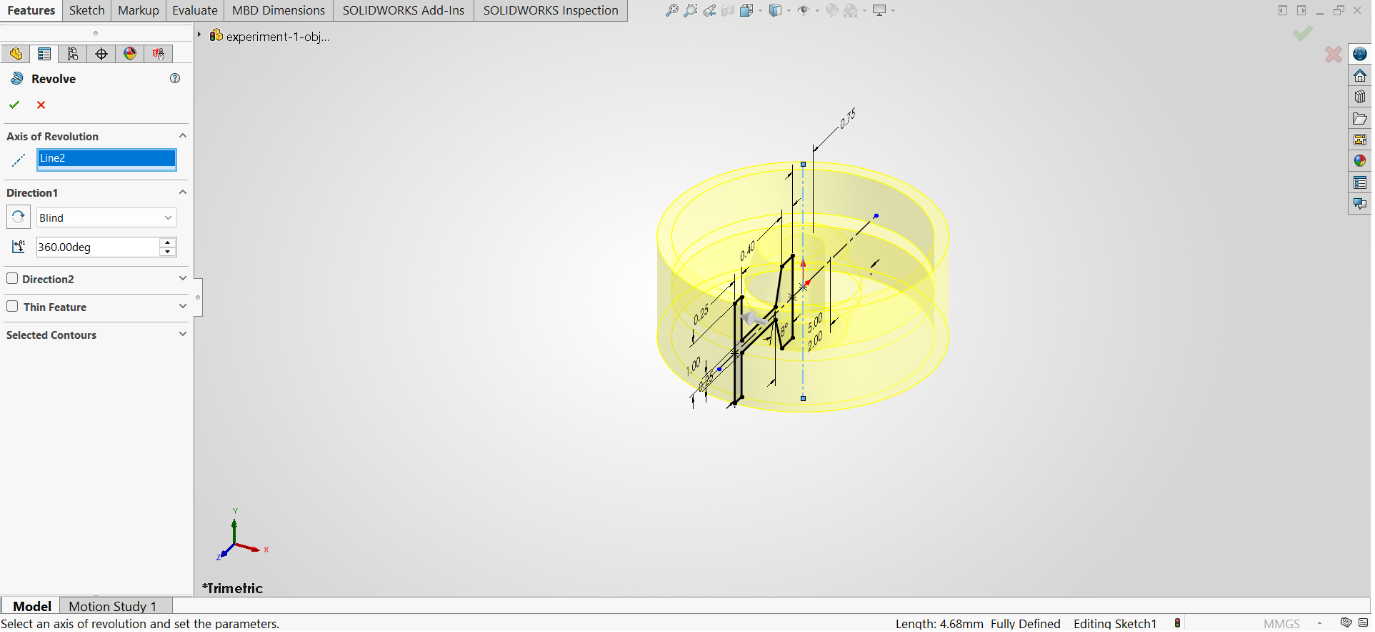
\includegraphics[width=\textwidth, keepaspectratio]{lab-01/assets/object-9/object-9-snap-2.png}
		\caption{Revolving the sketch around the vertical axis.}
	\end{subfigure}%
	\vspace{0.5em}
	\begin{subfigure}[b]{\textwidth}
		\centering
		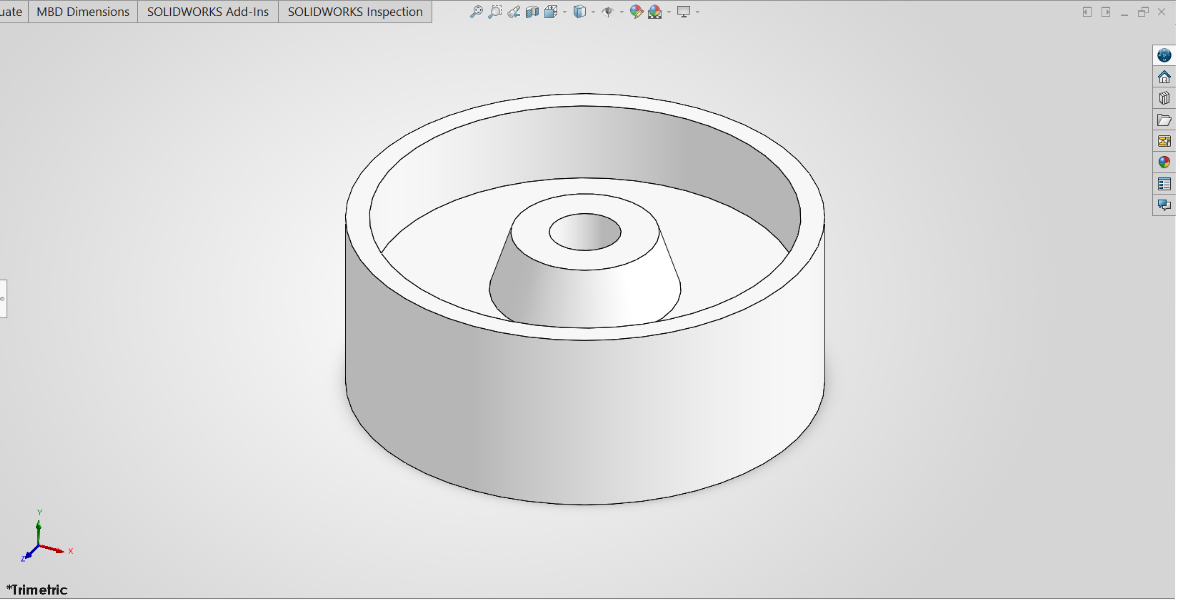
\includegraphics[width=\textwidth, keepaspectratio]{lab-01/assets/object-9/object-9-snap-3.png}
		\caption{Final Result.}
	\end{subfigure}

	\caption{Snapshots while Designing Object 9 in Solidworks}
	\label{lab01_object_9}
\end{figure}
